\chapter{Branch \& Bound}\label{branch_and_bound}

Come anticipato nel capitolo precedente possiamo usare due formulazioni (Cut Set o Subtour elimination) per risolvere il TSP. Il nostro problema però, sta nel avere un numero esponenziale di vincoli per garantire la connettività della soluzione. In questo capitolo descriviamo un modo per risolvere questo problema che viene anche descritto nel libro \cite{bertsimas}. Forniamo inoltre una nostra variazione dell’algoritmo derivante dall’analisi dell’efficienza di quello descritto nel libro.

\section{Branch \& Bound totale}

In questa sezione, presenteremo un algoritmo di branching che permette di ridurre il numero dei vincoli nel problema del TSP. L'algoritmo di branching è una tecnica di risoluzione che suddivide il problema originale in sottoproblemi più piccoli, riducendo in molti casi il costo della risoluzione. Nella nostra ambientazione del problema usiamo un grafo completo orientato quindi di seguito presentiamo brevemente la formulazione completa.

Con 4.a e 4.b ci assicuriamo che per ogni nodo ci sia esattamente un arco entrante e un arco uscente.
I vincoli 4.c ci garantiscono la connettività della soluzione in quanto impongono almeno un possibile cammino da un nodo ad ogni altro nodo e il loro numero è \begin{math}O(2^{|N|})\end{math}.

\[ x_{i_j} =
  \begin{cases}
    1       & \quad \text{se} \text{l'arco \begin{math}(i, j) \in E\end{math} fa parte del percorso ottimo}\\
    0  & \quad \text{altrimenti}
  \end{cases}
\]

\[
\text{minimize} \quad \sum_{i = 1}^{|N|}\sum_{j = 1}^{|N|} c_{i_j} x_{i_j}
\]

\begin{minipage}[t]{0.9\textwidth}
\[
\sum_{i = 1}^{|N|} x_{i_j} = 1, \quad  i = 1, \dots, |N| 
\]
\end{minipage}%
\begin{minipage}[t]{0.1\textwidth}
\vspace{0,4cm}
(4.a)
\end{minipage}

\begin{minipage}[t]{0.9\textwidth}
\[
\sum_{j = 1}^{|N|} x_{i_j} = 1, \quad  j = 1, \dots, |N|
\]
\end{minipage}%
\begin{minipage}[t]{0.1\textwidth}
\vspace{0,4cm}
(4.b)
\end{minipage}

\begin{minipage}[t]{0.9\textwidth}
\[
\sum_{(i, j) \in \delta^{+}(S)}  x_{i_j} \geq 1, \quad \forall S \subset N, S \ne \varnothing, S \ne N
\]
\end{minipage}%
\begin{minipage}[t]{0.1\textwidth}
\vspace{0,2cm}
(4.c)
\end{minipage}

\[
dove \quad \delta^{+}(S) = \{ (i,j) \in E: i \in S, j \notin S \}
\]

\begin{minipage}[t]{0.9\textwidth}
\[
x_a \in \{0, 1\}, \quad \forall a \in E
\]
\end{minipage}%
\begin{minipage}[t]{0.1\textwidth}
\vspace{0,1cm}
(4.d)
\end{minipage}

\subsection{Problema di assegnamento}
In \ref{elon_teletrasporto} (\nameref{elon_teletrasporto}) abbiamo già visto a cosa ci porta la rimozione dei vincoli di connessione. In particolare ci può portare ad una soluzione disconnessa e il problema restante prende il nome di Problema di Assegnamento (PA). La sua matrice dei vincoli è unimodulare e, quindi, la soluzione del rilassamento continuo è intera.

Possiamo procedere dicendo che la soluzione del PA sarà sicuramente un limite inferiore a quella del problema originale in quanto lo spazio ammissibile del TSP è compreso in quello del PA. Se la soluzione del PA produce un solo ciclo, allora sarà la soluzione ottima per il TSP, altrimenti si avrà un insieme di cicli disgiunti in cui ogni nodo è visitato esattamente una volta.

Possiamo quindi pensare di risolvere il TSP usando il Branch and Bound, in cui i limiti inferiori sono calcolati risolvendo dei problemi di assegnamento. 

Nel branching si fissano a zero le variabili che possono rendere inammissibile la soluzione per il TSP, quindi quelle con valore 1 della soluzione al PA.

Nella figura \ref{img:es_sol_disconnessa} notiamo che abbiamo due cicli nella soluzione per il PA. Il numero di nodi è 8, quindi creiamo 8 nodi figli e per ogni problema cerchiamo di aprire uno dei archi del percorso proposto dalla soluzione del PA.

Fortunatamente non si avrà la necessità di visitare, e quindi anche costruire, tutto l'albero, in quanto possiamo potare alcune sue parti a priori. In particolare un nodo non genera figli se:

\begin{itemize}
    \item se la soluzione per il PA è ammissibile per il TSP
    \item se la soluzione del PA è inammissibile
    \item se la soluzione del PA è inammissibile per il TSP ed è peggiore della migliore soluzione ammissibile per il TSP finora trovata
\end{itemize}

\newpage
Forniamo il pseudocodice dell'algoritmo che abbiamo sviluppato.

\begin{algorithm}
\caption{Branch and Bound for TSP}\label{alg:brand:and_bound_pseudocode}
\begin{algorithmic}
\State $best\_solution \gets None$
\State $best\_objective\_value \gets +\infty$
\State $stack \gets$ a list with only one model for PA
\While{$stack$ is not empty}
    \State $current\_model \gets stack.pop()$
    \State $solution \gets current\_model.solve()$
    \If{$solution$ is None}
        continue  \Comment{Infeasible solution, backtrack}
    \EndIf
    \State $objective\_value \gets solution.get\_objective\_value()$
    \If{$objective\_value \geq best\_objective\_value$}
        continue  \Comment{Solution is worse than the best found so far, backtrack}
    \EndIf
    \If{the number of cicles is 1}
        \State $best\_solution \gets solution$
        \State $best\_objective\_value \gets objective\_value$\\
        \quad \quad \quad continue\Comment{Found a feasible solution with lower objective value}
    \EndIf
    \For{$(i, j) \in (1\dots N) \times (1\dots N)$}
        \If{$i \ne j$ and $x_{i_j}$ is an arc in the current solution}
            \State Create a new model cloning the previous one
            \State Add constrain $x_{i_j} = 0$ to the new model
            \State Push the new model to the stack
        \EndIf
    \EndFor
\EndWhile
\If{$best\_solution$ is None}
        \State raise error "Infeasible"
\EndIf \\
\Return$best\_solution$
\end{algorithmic}
\end{algorithm}

\section{Branch \& Bound con branching parziale}
Dopo aver implementato l’algoritmo descritto nella sezione precedente abbiamo eseguito dei test. Pur ottenendo dei buoni risultati per alcuni casi di studio, tra questi abbiamo notato un degrado considerevole delle prestazioni. Dopo aver investigato sulla natura del problema abbiamo concluso che la principale causa sia una forte frammentazione dell’albero causata dalla generazione di \begin{math}|N| \end{math} figli ad ogni iterazione di branching. 

Proponiamo quindi un modo alternativo che sfrutta le stesse idee descritte prima, ma che esegue il branching solo su due variabili decisionali che nella soluzione corrente, non ammissibile del problema viaggiatore, rappresentano due degli archi scelti.

Precisiamo che la soluzione trovata con questo metodo potrebbe non essere ottima per il TSP in quanto si anulla la possibilità che i due archi, che si vanno a chiudere, capitino insime nella  soluzione finale. Questo non rappresenta un problema nel caso del branching totale (su tutti gli archi del percorso scelto) in quanto in questo caso particolare, se la soluzione corrente non è amissibile per il TSP, non potranno mai capitare tutti iniseme nella sua soluzione ottima. 

Da questa osservazione possiamo concludere che aumentando il numero dei rami uscenti da un nodo di branching si ha più possibilità di aviccinarci alla soluzione ottima per il TSP.

Inoltre, in seguito ad alcune prove, si è notato che la percentuale di incremento del costo rispetto alla soluzione ottima del TSP diminuisce, se si sceglie con cura gli archi da anullare. Nella nostra versione scegliamo quelli di costo maggiore fra quelli proposti dalla soluzione corrente. 

\section{Analisi}
Scorporiamo la nostra analisi su due concetti: l'aumento del costo con il branching binario e il tempo di esecuzione dei tre algoritmi.

Analizziamo prima l'incremento del costo nel caso del branching biario, con il quale si ha il rischio di non arrivare ad una soluzione ottima, ma si ha il vantaggio di una diramazione inferiore con conseguente incremento di efficienza.

In merito sono state create 30 istanze del problema con 15 nodi. Nella tabella \ref{tab:bb_incremento_costo} riportiamo per ogni algoritmo di branching il tempo di completamento, il numero dei nodi aggiunti ed il valore della funzione obiettivo all'ottimo. Nell'ultima colonna forniamo l'incremento del costo rispetto alla soluzione ottima del TSP. La soluzione ottima in questo caso è stata ottenuta con l'algoritmo che esegue il branching su tutti gli archi, ma per sicurezza è stata confrontata anche con quella ottenuta usando la formulazione di Miller–Tucker–Zemlin descritta nella sezione \ref{mtz} (\nameref{mtz}). Notiamo che pur essendoci dei casi dove la soluzione finale subisce un piccolo incremento, nella maggioranza dei casi si arriva alla stessa soluzione del branching totale.

\begin{table}[htbp]
    \centering
    \footnotesize
    \setlength{\tabcolsep}{2pt} 
    \renewcommand{\arraystretch}{1.2} 
    \begin{tabular}{|c|c|c|c|c|c|c|c|}
        \hline
        \textbf{ID} & \textbf{B\&B Time (s)} & \textbf{\# Added nodes} & \textbf{Obj Value} & \textbf{Binary B\&B Time (s)} & \textbf{\# Added nodes} & \textbf{Obj Value} & \textbf{Increase \%} \\
        \hline
        1 & 1.86 & 45 & 157 & 0.11 & 2 & 157 & 0.0 \% \\
        2 & 6.12 & 135 & 181 & 0.11 & 2 & 181 & 0.0 \% \\
        3 & 1.28 & 30 & 183.0 & 0.10 & 2 & 183.0 & 0.0 \% \\
        4 & 0.05 & 0 & 154 & 0.03 & 0 & 154 & 0.0 \% \\
        5 & 4.33 & 105 & 104 & 0.87 & 20 & 110 & 5.7\% \\
        6 & 1.97 & 45 & 158 & 0.21 & 4 & 158 & 0.0 \% \\
        7 & 7.63 & 165 & 187 & 2.36 & 48 & 202 & 8.0 \% \\
        8 & 0.12 & 0 & 138 & 0.04 & 0 & 138 & 0.0 \% \\
        9 & 0.1 & 0 & 187 & 0.03 & 0 & 187 & 0.0 \% \\
        10 & 3.96 & 90 & 181 & 1.41 & 32 & 205 & 13.26 \% \\
        11 & 7.15 & 165 & 143 & 0.58 & 12 & 150 & 4.9 \% \\
        12 & 0.06 & 0 & 195 & 0.03 & 0 & 195 & 0.0 \% \\
        13 & 18.02 & 390 & 163 & 0.66 & 12 & 163 & 0.0 \% \\
        14 & 5.43 & 120 & 202 & 0.12 & 2 & 203 & 0.5 \% \\
        15 & 4.03 & 90 & 158 & 0.12 & 2 & 158 & 0.0 \% \\
        16 & 0.09 & 0 & 225 & 0.03 & 0 & 225 & 0.0 \% \\
        17 & 1.94 & 45 & 187 & 1.2 & 26 & 195 & 4.28 \% \\
        18 & 0.05 & 0 & 177 & 0.03 & 0 & 177 & 0.0 \% \\
        19 & 12.85 & 285 & 166 & 0.5 & 10 & 178 & 7.23 \% \\
        20 & 0.05 & 0 & 147 & 0.03 & 0 & 147 & 0.0 \% \\
        21 & 0.09 & 0 & 102 & 0.03 & 0 & 102 & 0.0 \% \\
        22 & 5.4 & 120 & 217 & 0.49 & 10 & 217 & 0.0 \% \\
        23 & 0.09 & 0 & 121 & 0.03 & 0 & 121 & 0.0 \% \\
        24 & 3.28 & 75 & 133 & 0.26 & 4 & 135 & 1.5 \% \\
        25 & 13.98 & 300 & 161 & 1.49 & 30 & 162 & 0.62 \% \\
        26 & 1.3 & 30 & 157 & 0.11 & 2 & 157 & 0.0 \% \\
        27 & 0.05 & 0 & 171 & 0.03 & 0 & 171 & 0.0 \% \\
        28 & 0.05 & 0 & 148 & 0.03 & 0 & 148 & 0.0 \% \\
        29 & 4.7 & 105 & 151 & 0.12 & 2 & 151 & 0.0 \% \\
        30 & 11.46 & 255 & 158 & 0.32 & 6 & 158 & 0.0 \% \\
        \hline
    \end{tabular}
    \caption{I due Branch and Bound a confronto:\\
    per ogniuno dei due algoritmi riportiamo il tempo di complletamento in secondi, il numero dei nodi aggiunti e il risultato della funzione obiettivo all'ottimo. Nell'ultima colonna riportiamo la percentuale di incremento della funzione obiettivo}
    \label{tab:bb_incremento_costo}
\end{table}

\newpage

Nella tabella successiva \ref{tab:time_table} aggiungiamo anche il tempo di completamento per la formulazione MTZ.

Precisiamo che i risultati ottenuti con il branching totale rappresentano la soluzione ottima per il TSP e coincidono con la soluzione ottenuta usando la formulazione MTZ.

I tempi di esecuzione del B\&B Totale sono superiori a quelli di MTZ. Di conseguenza, è stata presa la decisione di confrontare la soluzione del rilassamento continuo di MTZ con la soluzione del Problema di Assegnamento. I risultati mostrano che per tutte le trenta, la soluzione all'ottimo rilassamento MTZ è superiore o uguale a quella ottenuta con PA. 

In particolare per le istanze 1, 2, 3, 6, 10, 11, 13, 14, 17, 22, 24, 25, 30 la soluzione del PA è maggiore di quella del rilassamento di MTZ (differenza compresa fra 0.57 e 3.64).

Quindi questo ci porta a dire che il rilassamento della formulazione di MTZ sia migliore di quello del PA. 

\begin{table}[htbp]
    \centering
    \begin{tabular}{|c|c|c|c|c|}
        \hline
        \textbf{ID} & \textbf{B\&B Time (s)} & \textbf{Binary B\&B Time (s)} & \textbf{MTZ Time (s)} \\
        \hline
        1 & 1.86 & 0.11 & 0.07 \\
2 & 6.12 & 0.11 & 0.03 \\
3 & 1.28 & 0.10 & 0.03 \\
4 & 0.05 & 0.03 & 0.01 \\
5 & 4.33 & 0.87 & 0.03 \\
6 & 1.97 & 0.21 & 0.03 \\
7 & 7.63 & 2.36 & 0.01 \\
8 & 0.12 & 0.04 & 0.02 \\
9 & 0.10 & 0.03 & 0.01 \\
10 & 3.96 & 1.41 & 0.03 \\
11 & 7.15 & 0.58 & 0.03 \\
12 & 0.06 & 0.03 & 0.01 \\
13 & 18.02 & 0.66 & 0.03 \\
14 & 5.43 & 0.12 & 0.03 \\
15 & 4.03 & 0.12 & 0.02 \\
16 & 0.09 & 0.03 & 0.01 \\
17 & 1.94 & 1.20 & 0.02 \\
18 & 0.05 & 0.03 & 0.01 \\
19 & 12.85 & 0.50 & 0.03 \\
20 & 0.05 & 0.03 & 0.01 \\
21 & 0.09 & 0.03 & 0.01 \\
22 & 5.40 & 0.49 & 0.05 \\
23 & 0.09 & 0.03 & 0.01 \\
24 & 3.28 & 0.26 & 0.02 \\
25 & 13.98 & 1.49 & 0.03 \\
26 & 1.30 & 0.11 & 0.01 \\
27 & 0.05 & 0.03 & 0.01 \\
28 & 0.05 & 0.03 & 0.01 \\
29 & 4.70 & 0.12 & 0.01 \\
30 & 11.46 & 0.32 & 0.03 \\
        \hline
    \end{tabular}
    \caption{Tempo di completamento per Branch and Bound totale, binario e per la formulazione MTZ}
    \label{tab:time_table}
\end{table}



\newpage
\section{Applicazione al caso di studio di Elon Musk}
Nella sezione precedente, abbiamo presentato come possiamo gestire il numero esponenziale di vincoli per garantire una soluzione connessa nel TSP tramite un algoritmo di branching. In questa sezione esaminiamo passo passo l’esecuzione dell'algoritmo di branching binario sulla nostra ambientazione del problema.

\subsection{Definizione del problema}

Consideriamo un grafo completo in cui i nodi rappresentano i pianeti del nostro sistema solare e gli archi rappresentano i percorsi tra i pianeti. Ogni arco ha associato un costo. L'obiettivo è determinare il percorso chiuso di costo minimo che permetta a Elon Musk di visitare tutti i pianeti una sola volta, tornando infine al pianeta di partenza.

Il grafo, nel nostro caso è un grafo orientato in quanto il costo può differire scambiando il pianeta di partenza e quello di arrivo. In particolare il costo del viaggio dipende dai seguenti fattori:

\begin{itemize}
    \item distanza
    \item numero degli asteroidi sul percorso
    \item orientazione della navicella rispetto alla direzione della luce (la navicella di Elon vuole sprecare meno energia elettrica possibile acquisendone il più possibile dai raggi solari)
\end{itemize}

\[
costo = w1 * dist\_norm + w2 * num\_ast\_norm + w3 * angolo\_trasformato 
\]

\[
dist\_norm = (distanza - distanza\_min) / (distanza\_max - distanza\_min)
\]

\[
num\_ast\_norm = (num\_ast - num\_ast_min) / (num\_ast\_max - num\_ast\_min)
\]

\[
angolo\_trasformato = angolo / 180^{\circ}
\]

dove w1, w2 e w3 rappresentano i pesi che diamo a ciascun parametro che influenza il costo finale.


\subsection{Esecuzione dell'algoritmo}
Andiamo a vedere le decisioni che prende l'algoritmo su ciascun nodo dell'albero. Rappresentiamo l'albero in Figura \ref{img:albero}, nel quale i nodi sono numerati nello stesso ordine nel quale vengono visitati.

\begin{itemize}
    \item Al nodo 1 come si può vedere nell'immagine \ref{img:es_space_sol_disconnessa} si ha una soluzione ammissibile per il PA, ma non per il TSP, quindi 117 è un limite inferiore alla soluzione del problema originario e si hanno due nuovi nodi: 2 e 3. Nelle fasi successive andiamo a migliorare sempre di più i limiti inferiori per poi raggiungere la soluzione ottima.
    \item Lo stesso avviene per i nodi 2 e 3. Hanno una soluzione ammissibile per il problema di PA, ma non per il TSP, quindi generano entrambi due figli.
    \item Il nodo 4 individua una soluzione ammissibile (rappresentata in figura \ref{img:es_space_sol_connessa}) per il problema di TSP, per ora è la soluzione migliore, quindi viene aggiornata. Siccome si ha una soluzione ammissibile per il problema di TSP, il nodo 4 non genera figli.
    \item Negli altri nodi (5, 6, 7) la soluzione è peggiore di quella che è stata già trovata al nodo 4, quindi non generano figli.
\end{itemize}

\begin{figure}[ht]
	\centering
	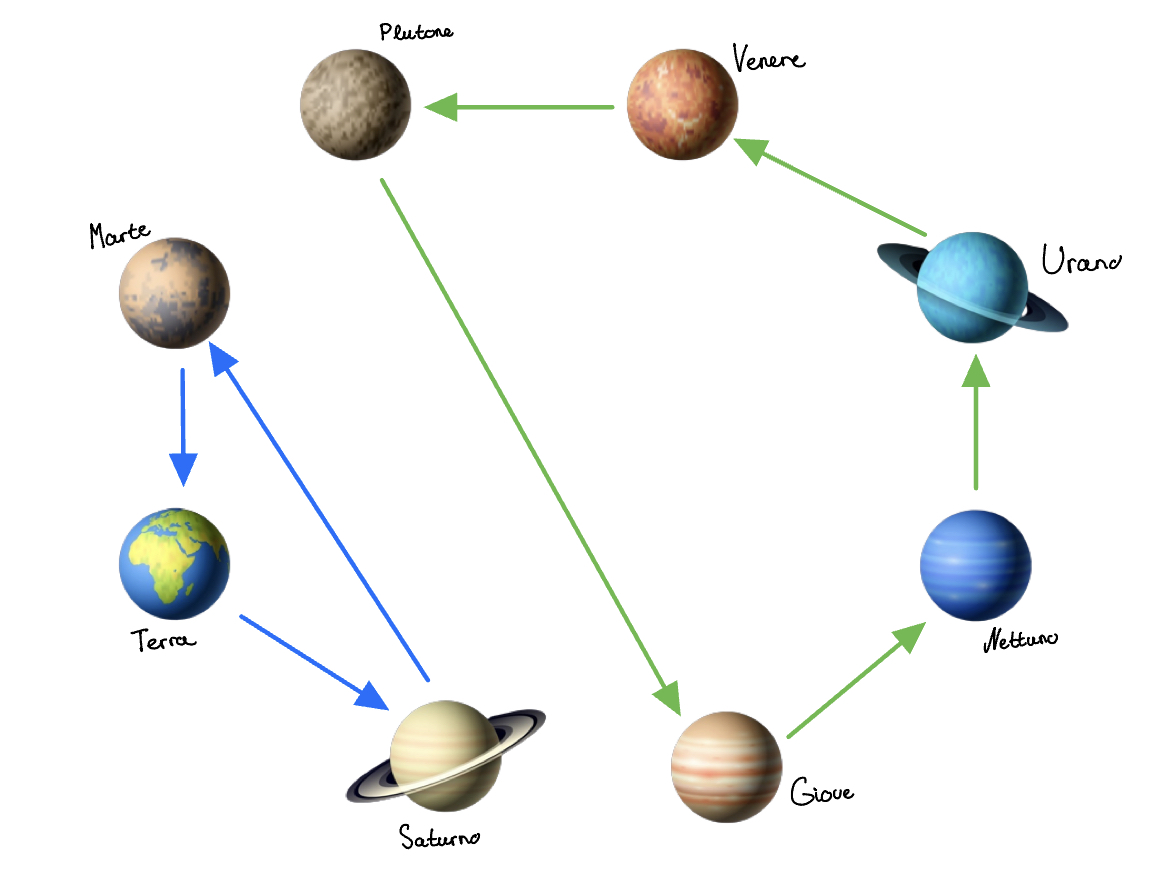
\includegraphics[width=1\columnwidth]{images/es_space_sol_disconnessa}
	\caption{\textit{Soluzione al problema di Assegnamento al Nodo 1}}
	\label{img:es_space_sol_disconnessa}
\end{figure}

\begin{figure}[ht]
	\centering
	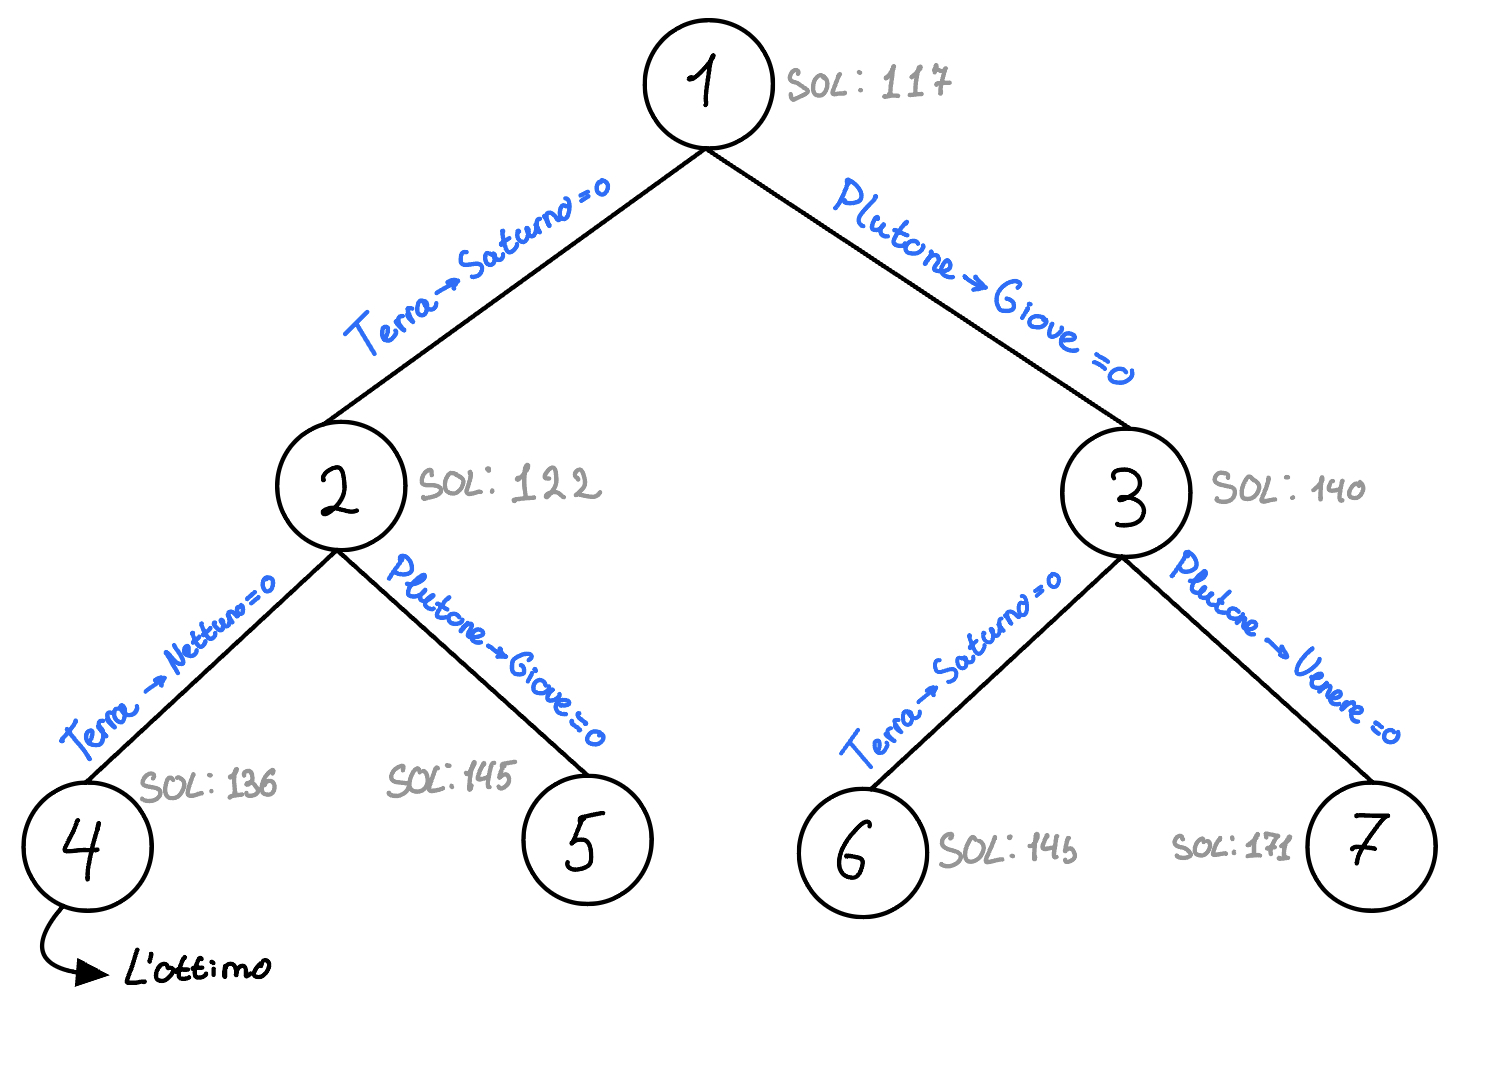
\includegraphics[width=1\columnwidth]{images/albero}
	\caption{\textit{Albero creato dall'algoritmo di branching}}
	\label{img:albero}
\end{figure}

\begin{figure}[ht]
	\centering
	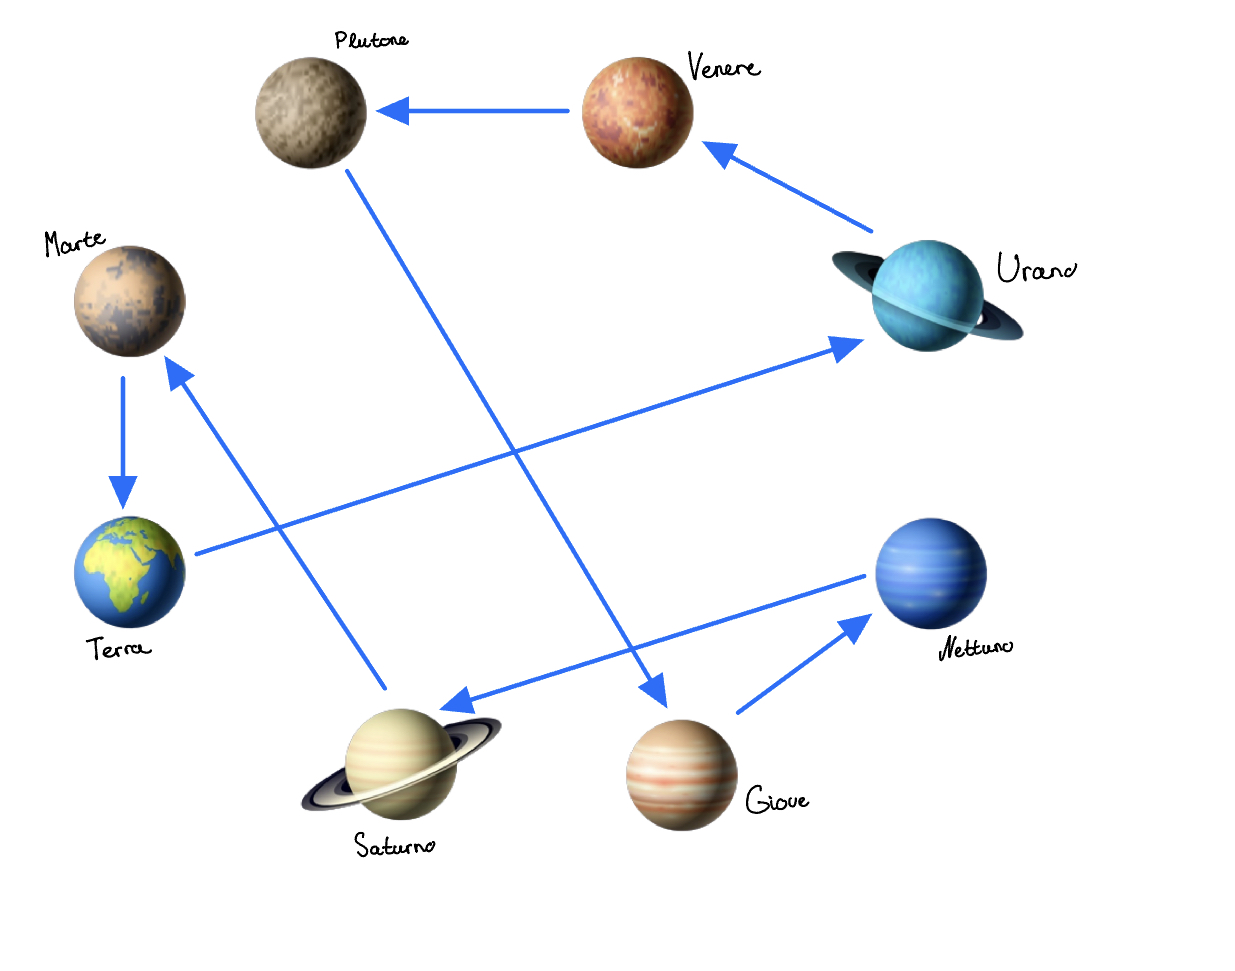
\includegraphics[width=1\columnwidth]{images/es_space_sol_connessa}
	\caption{\textit{Soluzione finale al problema del TSP}}
	\label{img:es_space_sol_connessa}
\end{figure}